\chapter{Related Work}\label{ch:related-work}

There exist lots of ways to visualize data and the relations between data. In this chapter, we discuss visualization techniques related to the needs of GuideaMaps 2.0 (\autoref{sec:visualization-techniques}). In \autoref{sec:existing-tools}, we discuss related tools.


% ------------------------------------
% ----- VISUALIZATION TECHNIQUES -----
% ------------------------------------
\section{Visualization Techniques}\label{sec:visualization-techniques}

% ---------------------
% ----- MIND MAPS -----
% ---------------------
\subsection{Mind Maps}\label{sec:mind-maps}
The most well-known technique to visualize related data is to create a mind map (a.k.a. idea map). This technique is mainly used to show the relation between portions of information and for brainstorming purposes. Other applications where this technique is used are note-taking, and problem solving. \citep{knowledgemapsbalaid} \\

Mind maps are created by writing the main idea in the middle of the drawing, while all sub-ideas are placed around that center node. Each sub-idea is connected with its parent by means of a line. Hence, this kind of visualization is not difficult to create or understand. Its simplicity is one of the reasons why it is used a lot in practice.\\

Because mind maps is not a new concept, but one that most people already know quite well, we will only discuss one important aspect about this visualization technique. When using a digital version of mind maps, in general, the user can change the position of the nodes. \cite{wiegmann-1992} state that maps taking the Gestalt principles \citep{koffka2013principles} into account would be more performance-effective than maps that don't integrate Gestalt principles. Therefore, digital mind map systems usually allow their users to re-organize the nodes using drag and drop and by changing the color of the nodes. In this way, the user can, for example, put nodes containing similar data closer to each other and give them the same color (proximity and similarity principle).



% ----------------------------
% ----- VISUAL METAPHORS -----
% ----------------------------
\subsection{Visual Metaphors}\label{sec:visual-metaphors}
Another technique that can be used to represent content is the use of visual metaphors.

\begin{quote}
``A visual metaphor is a graphic structure that uses the shape and elements of a familiar natural or manmade artefact or of an easily recognizable activity or story to organize content meaningfully and use the associations with the metaphor to convey additional meaning about the content.'' \hfill \citep{eppler-2006}
\end{quote}

This technique could be used if you want to help users to memorize the most important elements of a topic, method or concept. In that case, you have to choose a metaphor which has properties in common with the topic, concept or method. \citep{eppler-2006} An example of a visual metaphor is shown in \autoref{fig:visual-metaphor}. It shows ``a mixed visual metaphor/conceptual diagram template to structure learning content in a narrative structure during a class room discussion'' \citep{eppler-2006}. 

\begin{figure}[H]
	\centering
	\frame{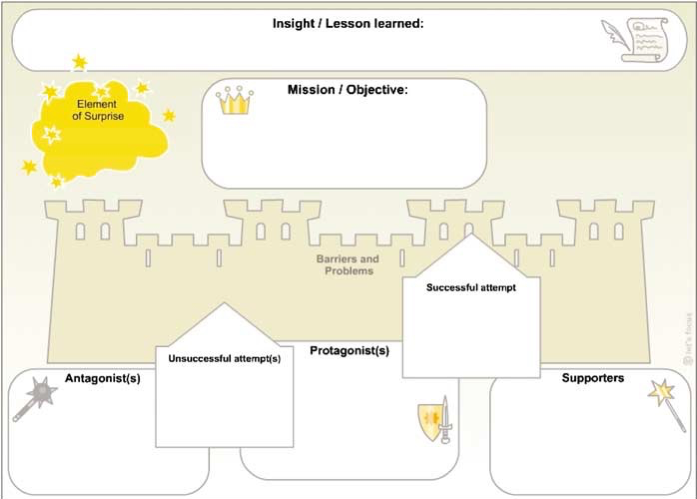
\includegraphics[width=0.75\linewidth]{relatedwork/visual-metaphor.png}}
	\caption{Example of a visual metaphor \citep{eppler-2006}.}
	\label{fig:visual-metaphor}
\end{figure}

As you can see in the figure, the visualization is completely adapted to the specific case of the topic. In this way, it is very difficult to create a generic metaphor, which can be used for different topics. As our tool should be usable for different topics, the technique of visual metaphors is less suitable for the needs of our tool.


% --------------------------
% ----- KNOWLEDGE MAPS -----
% --------------------------
\subsection{Knowledge Maps}\label{sec:knowledge-maps}
According to \cite{knowledgemapsbalaid}, \textit{knowledge maps} is an umbrella term for tools and techniques like mind maps. \cite{knowledgemapsodonnell} defined the concept as follows:

\begin{quote}
``Knowledge maps are node-link representations in which ideas are located in nodes and connected to other related ideas through a series of labeled links.'' \hfill 
\end{quote}

This way of representing information has for example a positive impact on students. The paper of \cite{knowledgemapsodonnell} teaches us that students using knowledge maps are better in remembering the main ideas of the subject in comparison to the ones that study from the text without the visualization. As GuideaMaps's purpose is more focused on representing large amounts of knowledge in an easy to grasp way, remembering the content is less important. However, the node-link representation with the main idea in the center also showed to be useful for this purpose, as illustrated by the popularity of mind maps.\\

Next to mind maps, concept maps is a second technique included under the umbrella of knowledge maps. Concept maps are in some sense similar to mind maps but they do have some different characteristics. First, the purpose of a mind map is to associate ideas, topics or things, while concept maps illustrate relations between concepts. Further, the structure of a concept map is mostly hierarchical and visualized like a tree. On the other hand, mind maps sometimes have a radial layout and not hierarchical. \citep{davies} An analysis by \cite{nesbit2006conceptmaps} showed that concept maps are more effective in grasping knowledge than reading long texts and being present in lectures, which is an analogous result to what \cite{knowledgemapsodonnell} showed us about knowledge maps. \\

Hence, we can state that GuideaMaps makes use of a knowledge map visualization and more specifically some kind of combination of mind maps and concept maps.



% --------------------------
% ----- EXISTING TOOLS -----
% --------------------------
\section{Existing Tools}\label{sec:existing-tools}
In this section, we will discuss several already existing tools with similar functionality as defined in the goals of our application.

\subsection{Browser-based}
To create a digital mind map, a lot of browser-based tools exist yet. They are all very similar and only differ in a small number of functionalities. Therefore, we only discuss two examples of such tools.\\

Bubbl.us\footnote{\url{https://bubbl.us/}} is an online mind-mapping tool with very interesting features. Because it is browser-based, it works on all platforms and devices. Furthermore, you do not have to download any software to be able to use it. The biggest drawback of the system is that the nodes only contain a title. It is impossible to provide some content in addition to the title of the node. Hence, this tool is probably only useful to write down simple ideas instead of more complex structures of related data. Another drawback is that you can only change the color of the nodes but you cannot customize their shape. But, as a user, you can drag and drop the nodes, share the visualization, work on it simultaneously, etc. Hence, Bubbl.us seems to be a well-created tool with lots of advantages. However, for the purpose of GuideaMaps 2.0, we need some functionality this tool does not provide.\\

A second browser-based tool is ``MindMeister''\footnote{\url{https://www.mindmeister.com/}}. It is very easy to create an account, on which your different visualizations can be stored. Users are allowed to drag and drop the nodes to other positions and change their layout in terms of color and borders. However, you cannot show a preview of the content in the node itself. You always have to click the node to be able to see the content. Further, it is not possible to customize the links, which can be a drawback because now they are represented as a solid line and it is not possible to add an arrow on them. As a consequence, this is a second well-created tool but missing some important functionality for GuideaMaps 2.0.


\subsection{Moodle}

\cite{scherl2012moodle} described Moodle as follows:
\begin{quote}
	``Moodle is a widely used learning management system. It visualizes inner and interdisciplinary relations between learning objects and is generated dynamically depending on user set parameters and interactions. It is a free open-source software package that provides a course management system for the implementation of internet-based learning environments.''
\end{quote}

In Moodle, navigation between courses only works by binding URLs to words or pictures, similar to the way Wikipedia does it. This way of linking resources makes it difficult to  ``stay on top of things''. Therefore, \cite{scherl2012moodle} extended Moodle to provide a clear orientation throughout navigation. In this extended version, new learning activities can be linked to already existing learning activities in any course present on the Moodle platform. In so-called concept map-based navigation, the students can open a full-screen concept map (example in \autoref{fig:moodle-concept-map}). Every node represents a learning object and a click on it opens the corresponding resource. Further, the currently visited learning object (node) is always in the center of the map, which is dynamically changed and updated based on user interactions. Hence, this system is comparable with the one we want to build: in our system, the currently selected node will be at the center as well and it should be possible to open nodes to see their content. However, important functionality is missing: similar to the browser-based examples, there is only a title visible for the nodes and no preview of the content. More important is that it is not possible to customize the layout of the nodes and the links, which is a requirement we certainly want to achieve in our solution.

\begin{figure}[H]
	\centering
	\frame{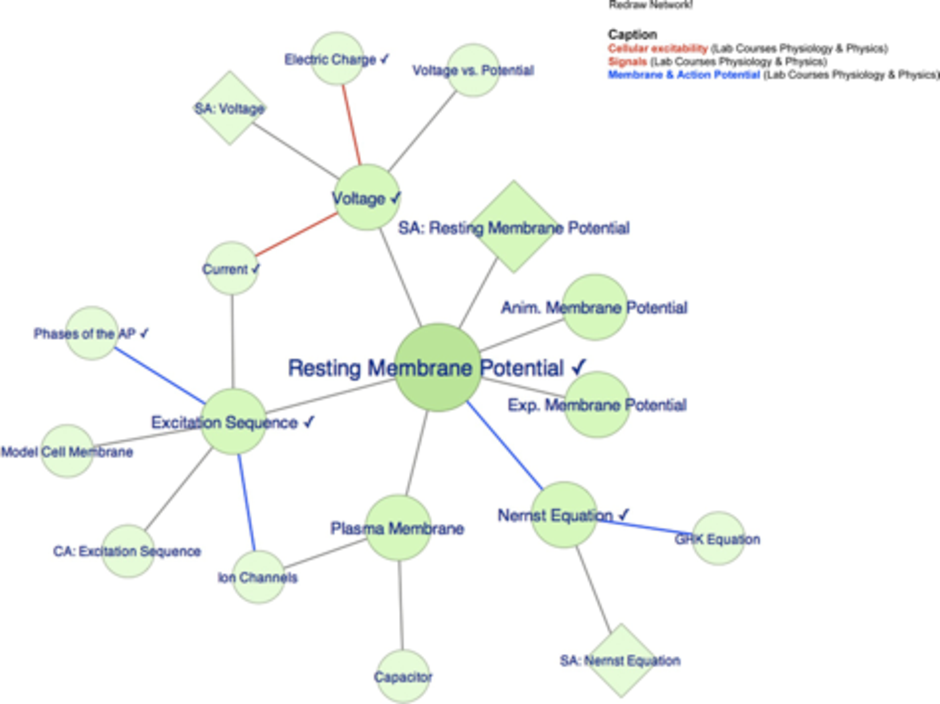
\includegraphics[width=0.75\linewidth]{relatedwork/moodle.pdf}}
	\caption{Example of concept map-based navigation in Moodle.}
	\label{fig:moodle-concept-map}
\end{figure}


\subsection{CmapTools}
\cite{novak2006conceptmapping} did the following:
\begin{quote}
	``Extending the use of concept mapping to other applications such as the integration of concept mapping with the World Wide Web (WWW) led to the development of software that enhanced the potential of concept mapping, evolving into the current version of CmapTools now used worldwide in schools, universities, corporations, and governmental and non-governmental agencies. CmapTools is a client-server software tool to facilitate the construction and sharing of concept maps.''
\end{quote}

\cite{canas2004conceptmapping} explain that CmapTools allows to publish knowledge models in concept map servers (CmapServers) and that these concept maps can be linked to related concept maps and to other types of media (e.g. images and web pages) in other servers. Further, the tool is also made collaborative. However, our own experience of experimenting with the software was a bit disappointing. The layout of the editor is quite old-fashioned and unsharp and the possibilities are not very clear. It seems new users have to spend some time to get used to the system. For our approach, we want to avoid such a situation, i.e. the possible actions in our application should be intuitive so that users do not lose time searching for the functionality they need. 







